%\documentclass[smaller, handout]{beamer}
\def\bmode{0} % Mode 0 for presentation, mode 1 for a handout with notes, mode 2 fo% r handout without notes
\if 0\bmode
\documentclass[smaller]{beamer}
\else \if 1\bmode
\immediate\write18{pdflatex -jobname=\jobname-Handout-Notes\space\jobname}
\documentclass[smaller,handout]{beamer}
\usepackage{handoutWithNotes}
\pgfpagesuselayout{2 on 1 with notes}[letterpaper, landscape, border shrink=4mm]
\else \if 2\bmode
\immediate\write18{pdflatex -jobname=\jobname-Handout\space\jobname}
\documentclass[smaller,handout]{beamer}
\fi
\fi
\fi

%%%%%%%%%%%%%%%%%%%%%%%%%%%%%%%%%%%%%%%%%%%%%%%%%%%%%%%%%%%%%%%%%%%%%%%%%%%%%%%%%%%%%%%%%%%%%
\newcommand{\coursetitle}{CEE 616: Probabilistic Machine Learning}
\newcommand{\longlecturetitle}{M3 Deep Neural Networks:\\ L3c: Neural Networks for Images}
\newcommand{\shortlecturetitle}{L3c: CNNs}
\newcommand{\instructor}{Jimi Oke}
\newcommand{\lecturedate}{Thu, Oct 23, 2025}
%%%%%%%%%%%%%%%%%%%%%%%%%%%%%%%%%%%%%%%%%%%%%%%%%%%%%%%%%%%%%%%%%%%%%%%%%%%%%%%%%%%%%%%%%%%%%

 
 
% \usepackage[T1]{fontenc} 
% \usepackage{lmodern} 
%\usepackage{etex}
 %\newcommand{\num}{6{} }

% \usetheme[
%   outer/progressbar=foot,
%   outer/numbering=fraction,
%   block=fill,
%   inner/subsectionpage=progressbar
% ]{metropolis}
\usetheme{Madrid}
\useoutertheme[subsection=false]{miniframes} % Alternatively: miniframes, infolines, split
\useinnertheme{circles}
% %\useoutertheme{Frankfurt}
% \usecolortheme{beaver}
% %\useoutertheme{crane}
% %\useoutertheme{metropolis}
\usepackage[backend=biber,style=authoryear,maxcitenames=2,maxbibnames=99,safeinputenc,url=false, eprint=false]{biblatex}
%\addbibresource{bib/references.bib}
% \AtEveryCitekey{\iffootnote{{\tiny}\tiny}{\tiny}}

% %\usepackage{pgfpages}
% %\setbeameroption{hide notes} % Only slides
% %\setbeameroption{show only notes} % Only notes
% %\setbeameroption{hide notes} % Only notes
% %\setbeameroption{show notes on second screen=right} % Both

% % \usepackage[sfdefault]{Fira Sans}

% % \setsansfont[BoldFont={Fira Sans}]{Fira Sans Light}
% % \setmonofont{Fira Mono}

% %\usepackage{fira}
% %\setsansfont{Fira}
% %\setmonofont{Fira Mono}
% % To give a presentation with the Skim reader (http://skim-app.sourceforge.net) on OSX so
% % that you see the notes on your laptop and the slides on the projector, do the following:
% % 
% % 1. Generate just the presentation (hide notes) and save to slides.pdf
% % 2. Generate onlt the notes (show only nodes) and save to notes.pdf
% % 3. With Skim open both slides.pdf and notes.pdf
% % 4. Click on slides.pdf to bring it to front.
% % 5. In Skim, under "View -> Presentation Option -> Synhcronized Noted Document"
% %    select notes.pdf.
% % 6. Now as you move around in slides.pdf the notes.pdf file will follow you.
% % 7. Arrange windows so that notes.pdf is in full screen mode on your laptop
% %    and slides.pdf is in presentation mode on the projector.

% % Give a slight yellow tint to the notes page
% \setbeamertemplate{note page}{\pagecolor{yellow!5}\insertnote}\usepackage{palatino}

% %\usetheme{metropolis}
% %\usecolortheme{beaver}
 \usepackage{tipa}
% \usepackage{enumerate}
\definecolor{darkcandyapplered}{HTML}{A40000}
\definecolor{lightcandyapplered}{HTML}{e74c3c}

% %\setbeamercolor{title}{fg=darkcandyapplered}

% \definecolor{UBCblue}{rgb}{0.04706, 0.13725, 0.26667} % UBC Blue (primary)
% \definecolor{UBCgrey}{rgb}{0.3686, 0.5255, 0.6235} % UBC Grey (secondary)

% % \setbeamercolor{palette primary}{bg=darkcandyapplered,fg=white}
% % \setbeamercolor{palette secondary}{bg=darkcandyapplered,fg=white}
% % \setbeamercolor{palette tertiary}{bg=darkcandyapplered,fg=white}
% % \setbeamercolor{palette quaternary}{bg=darkcandyapplered,fg=white}
% % \setbeamercolor{structure}{fg=darkcandyapplered} % itemize, enumerate, etc
% % \setbeamercolor{section in toc}{fg=darkcandyapplered} % TOC sections
% % \setbeamercolor{frametitle}{fg=darkcandyapplered,bg=white} % TOC sections
% % \setbeamercolor{title in head/foot}{bg=white,fg=white} % TOC sections
% % \setbeamercolor{button}{fg=darkcandyapplered} % TOC sections

% % % Override palette coloring with secondary
% % \setbeamercolor{subsection in head/foot}{bg=lightcandyapplered,fg=white}

%\usecolortheme{crane}
% \makeatletter
% \setbeamertemplate{headline}{%
%   \begin{beamercolorbox}[colsep=1.5pt]{upper separation line head}
%   \end{beamercolorbox}
%   \begin{beamercolorbox}{section in head/foot}
%     \vskip1pt\insertsectionnavigationhorizontal{\paperwidth}{}{}\vskip1pt
%   \end{beamercolorbox}%
%   \ifbeamer@theme@subsection%
%     \begin{beamercolorbox}[colsep=1.5pt]{middle separation line head}
%     \end{beamercolorbox}
%     \begin{beamercolorbox}[ht=2.5ex,dp=1.125ex,%
%       leftskip=.3cm,rightskip=.3cm plus1fil]{subsection in head/foot}
%       \usebeamerfont{subsection in head/foot}\insertsubsectionhead
%     \end{beamercolorbox}%
%   \fi%
%   \begin{beamercolorbox}[colsep=1.5pt]{lower separation line head}
%   \end{beamercolorbox}
% }
% \makeatother

% Reduce size of frame box
\setbeamertemplate{frametitle}{%
    \nointerlineskip%
    \begin{beamercolorbox}[wd=\paperwidth,ht=2.0ex,dp=0.6ex]{frametitle}
        \hspace*{1ex}\insertframetitle%
    \end{beamercolorbox}%
}


%\setbeamercolor{frametitle}{bg=darkcandyapplered!80!black!90!white}
%\setbeamertemplate{frametitle}{\bf\insertframetitle}

%\setbeamercolor{footnote mark}{fg=darkcandyapplered}
%\setbeamercolor{footnote}{fg=darkcandyapplered!70}
%\Raggedbottom
%\setbeamerfont{page number in head/foot}{size=\tiny}
%\usepackage[tracking]{microtype}


% %\usepackage[sc,osf]{mathpazo}   % With old-style figures and real smallcaps.
% %\linespread{1.025}              % Palatino leads a little more leading

% % Euler for math and numbers
% %\usepackage[euler-digits,small]{eulervm}
% %\AtBeginDocument{\renewcommand{\hbar}{\hslash}}
\usepackage{graphicx,multirow,booktabs}
\usepackage{animate}
\usepackage{media9}


% %\mode<presentation> { \setbeamercovered{transparent} }

\setbeamertemplate{navigation symbols}{}
\makeatletter
\def\beamerorig@set@color{%
  \pdfliteral{\current@color}%
  \aftergroup\reset@color
}
\def\beamerorig@reset@color{\pdfliteral{\current@color}}
\makeatother


% %=== GRAPHICS PATH ===========
\graphicspath{{./m3-images/}}
% % Marginpar width
% %Marginpar width
% %\setlength{\marginparsep}{.02in}


% %% Captions
% % \usepackage{caption}
% % \captionsetup{
% %   labelsep=quad,
% %   justification=raggedright,
% %   labelfont=sc
% % }

% \setbeamerfont{caption}{size=\footnotesize}
% \setbeamercolor{caption name}{fg=darkcandyapplered}

% %AMS-TeX packages

\usepackage{amssymb,amsmath,amsthm,mathtools} 
\usepackage{bm}
\DeclareMathOperator*{\argmax}{arg\,max}
\DeclareMathOperator*{\argmin}{arg\,min}
% \usepackage{color}

% %https://tex.stackexchange.com/a/31370/2269
\usepackage{mathtools,cancel}

\renewcommand{\CancelColor}{\color{red}} %change cancel color to red

\makeatletter
\let\my@cancelto\cancelto %copy over the original cancelto command
\newcommand<>{\cancelto}[2]{\alt#3{\my@cancelto{#1}{#2}}{\mathrlap{#2}\phantom{\my@cancelto{#1}{#2}}}}
% redefine the cancelto command, using \phantom to assure that the
% result doesn't wiggle up and down with and without the arrow
\makeatother


% %\usepackage{comment}
% %\usepackage{hyperref,enumerate}
% \usepackage{minitoc,array}

% \definecolor{slblue}{rgb}{0,.3,.62}
% % \hypersetup{
% %     colorlinks,%
% %     citecolor=blue,%
% %     filecolor=blue,%
% %     linkcolor=blue,
% %     urlcolor=slblue
% % }

% \usepackage{epstopdf}
% \epstopdfDeclareGraphicsRule{.gif}{png}{.png}{convert gif:#1 png:\OutputFile}
% \AppendGraphicsExtensions{.gif}

% %\usepackage{listings}

% %%% TIKZ
% \usepackage{forest}
\usepackage{tikz}
\usepackage{pgfplots}
\usepackage{pgfplotstable}
\usepackage{neuralnetwork}
%\usepackage{pgfgantt}
\pgfplotsset{compat=newest}

\usetikzlibrary{fit,arrows,shapes,positioning,shapes.geometric}
\usetikzlibrary{decorations.markings}
\usetikzlibrary{shadows,automata}
\usetikzlibrary{patterns}
\usetikzlibrary{trees,mindmap,backgrounds}
%\usetikzlibrary{circuits.ee.IEC}
\usetikzlibrary{decorations.text}
% % For Sagnac Picture
% \usetikzlibrary{%
%     decorations.pathreplacing,%
%     decorations.pathmorphing%
% }
% \tikzset{no shadows/.style={general shadow/.style=}}
% %
% %\usepackage{paralist}

% \tikzset{
%   font=\Large\sffamily\bfseries,
%   red arrow/.style={
%     midway,red,sloped,fill, minimum height=3cm, single arrow, single arrow head extend=.5cm, single arrow head indent=.25cm,xscale=0.3,yscale=0.15,
%     allow upside down
%   },
%   black arrow/.style 2 args={-stealth, shorten >=#1, shorten <=#2},
%   black arrow/.default={1mm}{1mm},
%   tree box/.style={draw, rounded corners, inner sep=1em},
%   node box/.style={white, draw=black, text=black, rectangle, rounded corners},
% }

% %%% FORMAT PYTHON CODE
% %\usepackage{listings}
% % Default fixed font does not support bold face
% \DeclareFixedFont{\ttb}{T1}{txtt}{bx}{n}{8} % for bold
% \DeclareFixedFont{\ttm}{T1}{txtt}{m}{n}{8}  % for normal

% % Custom colors
% \definecolor{deepblue}{rgb}{0,0,0.5}
% \definecolor{deepred}{rgb}{0.6,0,0}
% \definecolor{deepgreen}{rgb}{0,0.5,0}

% %\usepackage{animate}

% % Python style for highlighting
% % \newcommand\pythonstyle{\lstset{
% % language=Python,
% % basicstyle=\footnotesize\ttm,
% % otherkeywords={self},             % Add keywords here
% % keywordstyle=\footnotesize\ttb\color{deepblue},
% % emph={MyClass,__init__},          % Custom highlighting
% % emphstyle=\footnotesize\ttb\color{deepred},    % Custom highlighting style
% % stringstyle=\color{deepgreen},
% % frame=tb,                         % Any extra options here
%     % showstringspaces=false            % 
% % }}

% % % Python environment
% % \lstnewenvironment{python}[1][]
% % {
% % \pythonstyle
% % \lstset{#1}
% % }
% % {}

% % % Python for external files
% % \newcommand\pythonexternal[2][]{{
% % \pythonstyle
% % \lstinputlisting[#1]{#2}}}

% % Python for inline
% % 
% % \newcommand\pythoninline[1]{{\pythonstyle\lstinline!#1!}}

% %\usepackage{algorithm2e}

\newcommand{\eps}{\epsilon}
\newcommand{\bX}{\mb X}
\newcommand{\by}{\mb y}
\newcommand{\bbe}{\bm\beta}
\newcommand{\beps}{\bm\epsilon}
\newcommand{\bY}{\mb Y}

\newcommand{\osn}{\oldstylenums}
\newcommand{\dg}{^{\circ}}
\newcommand{\lt}{\left}
\newcommand{\rt}{\right}
\newcommand{\pt}{\phantom}
\newcommand{\tf}{\therefore}
\newcommand{\?}{\stackrel{?}{=}}
\newcommand{\fr}{\frac}
\newcommand{\dfr}{\dfrac}
\newcommand{\ul}{\underline}
\newcommand{\tn}{\tabularnewline}
\newcommand{\nl}{\newline}
\newcommand\relph[1]{\mathrel{\phantom{#1}}}
\newcommand{\cm}{\checkmark}
\newcommand{\ol}{\overline}
\newcommand{\rd}{\color{red}}
\newcommand{\bl}{\color{blue}}
\newcommand{\pl}{\color{purple}}
\newcommand{\og}{\color{orange!90!black}}
\newcommand{\gr}{\color{green!40!black}}
\newcommand{\dca}{\color{darkcandyapplered}}
\newcommand{\nin}{\noindent}
\newcommand*\circled[1]{\tikz[baseline=(char.base)]{
            \node[shape=circle,draw,thick,inner sep=1pt] (char) {\small #1};}}

\newcommand{\bc}{\begin{compactenum}[\quad--]}
\newcommand{\ec}{\end{compactenum}}

\newcommand{\p}{\partial}
\newcommand{\pd}[2]{\frac{\partial{#1}}{\partial{#2}}}
\newcommand{\dpd}[2]{\dfrac{\partial{#1}}{\partial{#2}}}
\newcommand{\pdd}[2]{\frac{\partial^2{#1}}{\partial{#2}^2}}
\newcommand{\pde}[3]{\frac{\partial^2{#1}}{\partial{#2}\partial{#3}}}
\newcommand{\nmfr}[3]{\Phi\left(\frac{{#1} - {#2}}{#3}\right)}
\newcommand{\Err}{\text{Err}}
\newcommand{\err}{\text{err}}

%\DeclarePairedDelimiter\ceil{\lceil}{\rceil}
%\DeclarePairedDelimiter\floor{\lfloor}{\rfloor}

%%%% GREEK LETTER SHORTCUTS %%%%%
\newcommand{\la}{\lambda}
\renewcommand{\th}{\theta}
\newcommand{\al}{\alpha}
\newcommand{\G}{\Gamma}
\newcommand{\si}{\sigma}
\newcommand{\Si}{\Sigma}


\pgfmathdeclarefunction{poiss}{1}{%
  \pgfmathparse{(#1^x)*exp(-#1)/(x!)}%
  }

\pgfmathdeclarefunction{gauss}{2}{%
  \pgfmathparse{1/(#2*sqrt(2*pi))*exp(-((x-#1)^2)/(2*#2^2))}%
}

\pgfmathdeclarefunction{expo}{2}{%
  \pgfmathparse{#1*exp(-#1*#2)}%
}

\pgfmathdeclarefunction{expocdf}{2}{%
  \pgfmathparse{1 -exp(-#1*#2)}%
}

\newcommand{\mb}{\mathbb}
\newcommand{\mc}{\mathcal}
\newcommand{\tr}{^{\top}}
\newcommand{\pe}{\pause}
% \usepackage{pst-plot}

% \usepackage{pstricks-add}
% \usepackage{auto-pst-pdf}   

% \psset{unit = 3}

% \def\target(#1,#2){%
%  {\psset{fillstyle = solid}
%   \rput(#1,#2){%
%     \pscircle[fillcolor = white](0.7,0.7){0.7}
%     \pscircle[fillcolor = blue!60](0.7,0.7){0.5}
%     \pscircle[fillcolor = white](0.7,0.7){0.3}
%     \pscircle[fillcolor = red!80](0.7,0.7){0.1}}}}
% \def\dots[#1](#2,#3){%
%     \psRandom[
%       dotsize = 2pt,
%       randomPoints = 25
%     ](!#2 #1 0.04 sub sub #3 #1 0.04 sub sub)%
%      (!#2 #1 0.04 sub add #3 #1 0.04 sub add)%
%      {\pscircle[linestyle = none](#2,#3){#1}}}


%%%%%%%%%%%%%%%%%%%%%%%%%%%%%%%%%%%%%%%%%%%%%%%%%%%
%%%%%%%%%%%%%%%%%%%%%%%%%%%%%%%%%%%%%%%%%%%%%%%%%%%
\title[\shortlecturetitle]{ {\normalsize \coursetitle}
  \\ \longlecturetitle}
\date[\lecturedate]{\footnotesize \lecturedate}
\author{{\bf \instructor}}
\institute[UMass Amherst]{
%\titlegraphic{\hfill
  \begin{tikzpicture}[baseline=(current bounding box.center)]
    \node[anchor=base] at (-7,0) (its) {
\includegraphics[scale=.3]{UMassEngineering_vert}} ;
  \end{tikzpicture}
  % \hfill\includegraphics[height=1.5cm]{logo}
}

%https://tex.stackexchange.com/questions/55806/mindmap-tikzpicture-in-beamer-reveal-step-by-step
  \tikzset{
    invisible/.style={opacity=0},
    visible on/.style={alt={#1{}{invisible}}},
    alt/.code args={<#1>#2#3}{%
      \alt<#1>{\pgfkeysalso{#2}}{\pgfkeysalso{#3}} % \pgfkeysalso doesn't change the path
    },
  }


% https://tex.stackexchange.com/questions/446468/labels-with-arrows-for-an-equation
% https://tex.stackexchange.com/a/402466/121799
\newcommand{\tikzmark}[3][]{
\ifmmode
\tikz[remember picture,baseline=(#2.base)] \node [inner sep=0pt,#1](#2) {$#3$};
\else
\tikz[remember picture,baseline=(#2.base)] \node [inner sep=0pt,#1](#2) {#3};
\fi
}

% \lstset{language=matlab,
%                 basicstyle=\scriptsize\ttfamily,
%                 keywordstyle=\color{blue}\ttfamily,
%                 stringstyle=\color{blue}\ttfamily,
%                 commentstyle=\color{gray}\ttfamily,
%                 morecomment=[l][\color{gray}]{\#}
%               }


%%% Local Variables:
%%% mode: latex
%%% TeX-master: t
%%% End:

%\usepackage{MnSymbol}              
\begin{document}
\maketitle
\begin{frame}
  \frametitle{Outline}
  \tableofcontents
\end{frame}

  

 
 
\section{Introduction}
\begin{frame}
  \frametitle{The convolutional neural network (CNN)}
  \pause

\visible<+->{  \begin{figure}
    \centering
    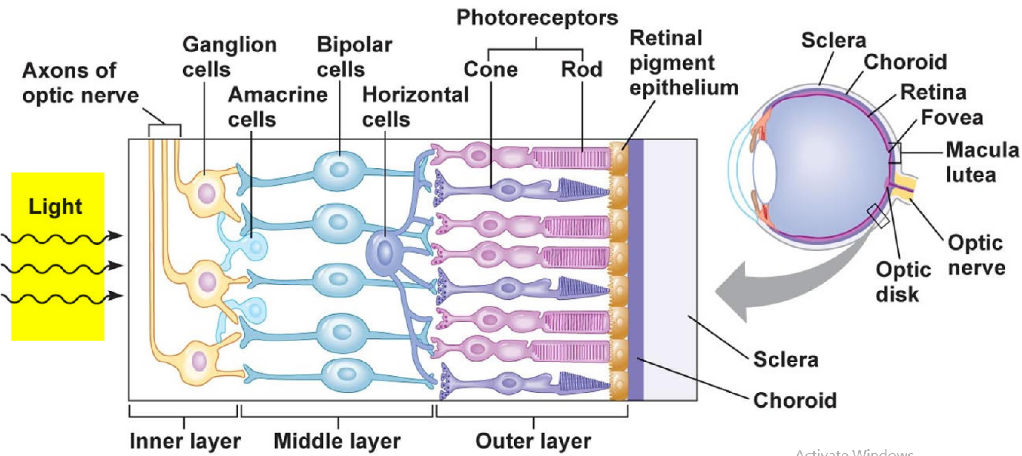
\includegraphics[width=.8\textwidth]{eye}

    {\scriptsize Source: \url{https://s3mn.mnimgs.com/img/shared/content_ck_images/ck_5ab694d5e73f4.png}}
\end{figure}}

  \begin{itemize}[<+->]
  \item Motivated by the image recognition process of the brain's visual cortex.

  \item Groundbreaking study showed that \textit{local receptive fields}  activate neurons
    in the visual cortex. (Hubel \& Wiesel, 1958; \href{https://www.ncbi.nlm.nih.gov/pmc/articles/PMC1363130/pdf/jphysiol01298-0128.pdf}{1959})

  \item Earliest neural network for image recognitron introduced \href{https://www.rctn.org/bruno/public/papers/Fukushima1980.pdf}{(Fukushima, 1980)}

  \item Milestone: introduction of \textit{LeNet-5} architecture for handwritten digit recognition \href{http://yann.lecun.com/exdb/publis/pdf/lecun-98.pdf}{(Yann LeCun et al., 1998)}
  \end{itemize}
  
\end{frame}


\begin{frame}
  \frametitle{Building blocks of a CNN}
  \pause
  \begin{itemize}[<+->]
  \item \textbf{Input layer:} the image to be classified 
  \item \textbf{Convolutional layer:} represents the action of a filter transmitting signals (features) from various
    portions (receptive fields) of the preceding layer. The size of the receptive field is specified by the
    \textit{convolutional kernel}. Each layer can have multiple feature maps representing different filters.
  \item \textbf{Pooling layer:} subsamples signals from preceding layer to reduce dimensionality and extract dominant
    features (subsample space determined by kernel size)
  \item \textbf{Dense layer:} neuron outputs are flattened and fully connected %(usually with decreasing number of neurons)
  \item \textbf{Output layer:} neurons equal to number of classes; with softmax activation
  \end{itemize}

  \visible<+->{
  \begin{center}
    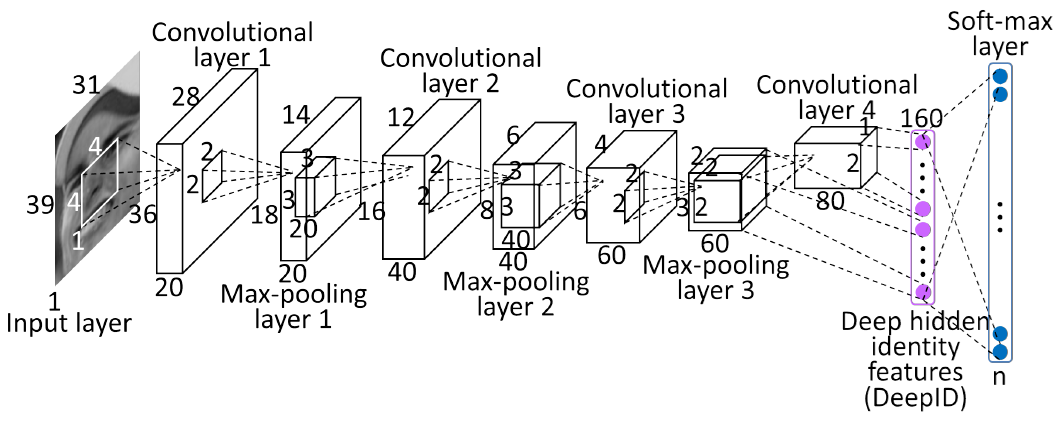
\includegraphics[width=.6\textwidth]{cnn-ex1}
  \end{center}

  {\tiny Source: \url{https://neurdiness.wordpress.com/2018/05/17/deep-convolutional-neural-networks-as-models-of-the-visual-system-qa/}}
}
  
\end{frame}

\section{Convolution}
\begin{frame}
  \frametitle{Convolution}
  \pause
  A convolution is a mathematical operation that computes the  overlap of a function $\rd g$ as it shifts across a function $\bl f$. \pause

  \medskip
  
  Thus, the convolution of $\bl f$ and $\rd g$ in the interval $[0,t]$ is given by: \pause
  
  \begin{equation}
    (f\circledast g)(t) =\pause \int {\bl f}(\tau){\rd g} (t - \tau)d\tau
  \end{equation}
  \pause

  Watch this animation for a better understanding: \url{https://youtu.be/C1N55M1VD2o}

  \bigskip
  
  In CNN terminology: \pause
  \begin{itemize}
  \item The function $\bl f$ is the \textbf{\bl input}
  \item The function $\rd g$ is the \textbf{\rd kernel}
  \item The convolution (or output) is called the \textbf{\pl feature map}
  \end{itemize}
\end{frame}

\begin{frame}
  \frametitle{Convolution (cont.)}
  \pause
  The convolution operation is commutative: \pause
  \begin{equation}
    (f\circledast g)(t) = \pause (g\circledast f)(t)
  \end{equation}
  \pause
    In CNNs, convolutions are typically
    \pause
    \begin{itemize}
    \item performed on a 2D image $I$ (input) \pause
    \item using a 2D kernel $K$ (dimensions $M\times N$)\pause
    \end{itemize}
    Thus, the discrete 2D convolution is given by: \pause
    \begin{equation}
      (I\circledast K)(i,j) = \pause\sum_{m=0}^{M-1}\sum_{n=0}^{N-1}I(m,n)K(i-m,j-n)
    \end{equation}
    \pause
    By the commutative property, we can write \pause
    \begin{equation}
      (K\circledast I)(i,j) = \pause\sum_{m=0}^{M-1}\sum_{n=0}^{N-1}I(i-m,j-n)K(m,n)
    \end{equation} \pause
    which is more straightforward to compute (the kernel is \textit{flipped} relative to the input)
  
\end{frame}



\begin{frame}
  \frametitle{Convolution and cross-correlation}
  In reality, NN libraries typically compute the \textbf{cross-correlation}:
  \pause
  \begin{equation}
    (K*I)(i,j) = \pause\sum_{m=0}^{M-1}\sum_{n=0}^{N-1}I(i+m, j+n)K(m,n)
  \end{equation}
  \pause
  which is equivalent to convolution performed without \textit{kernel flipping}.
  \pause
  \visible<+->{  \begin{figure}
      \centering
      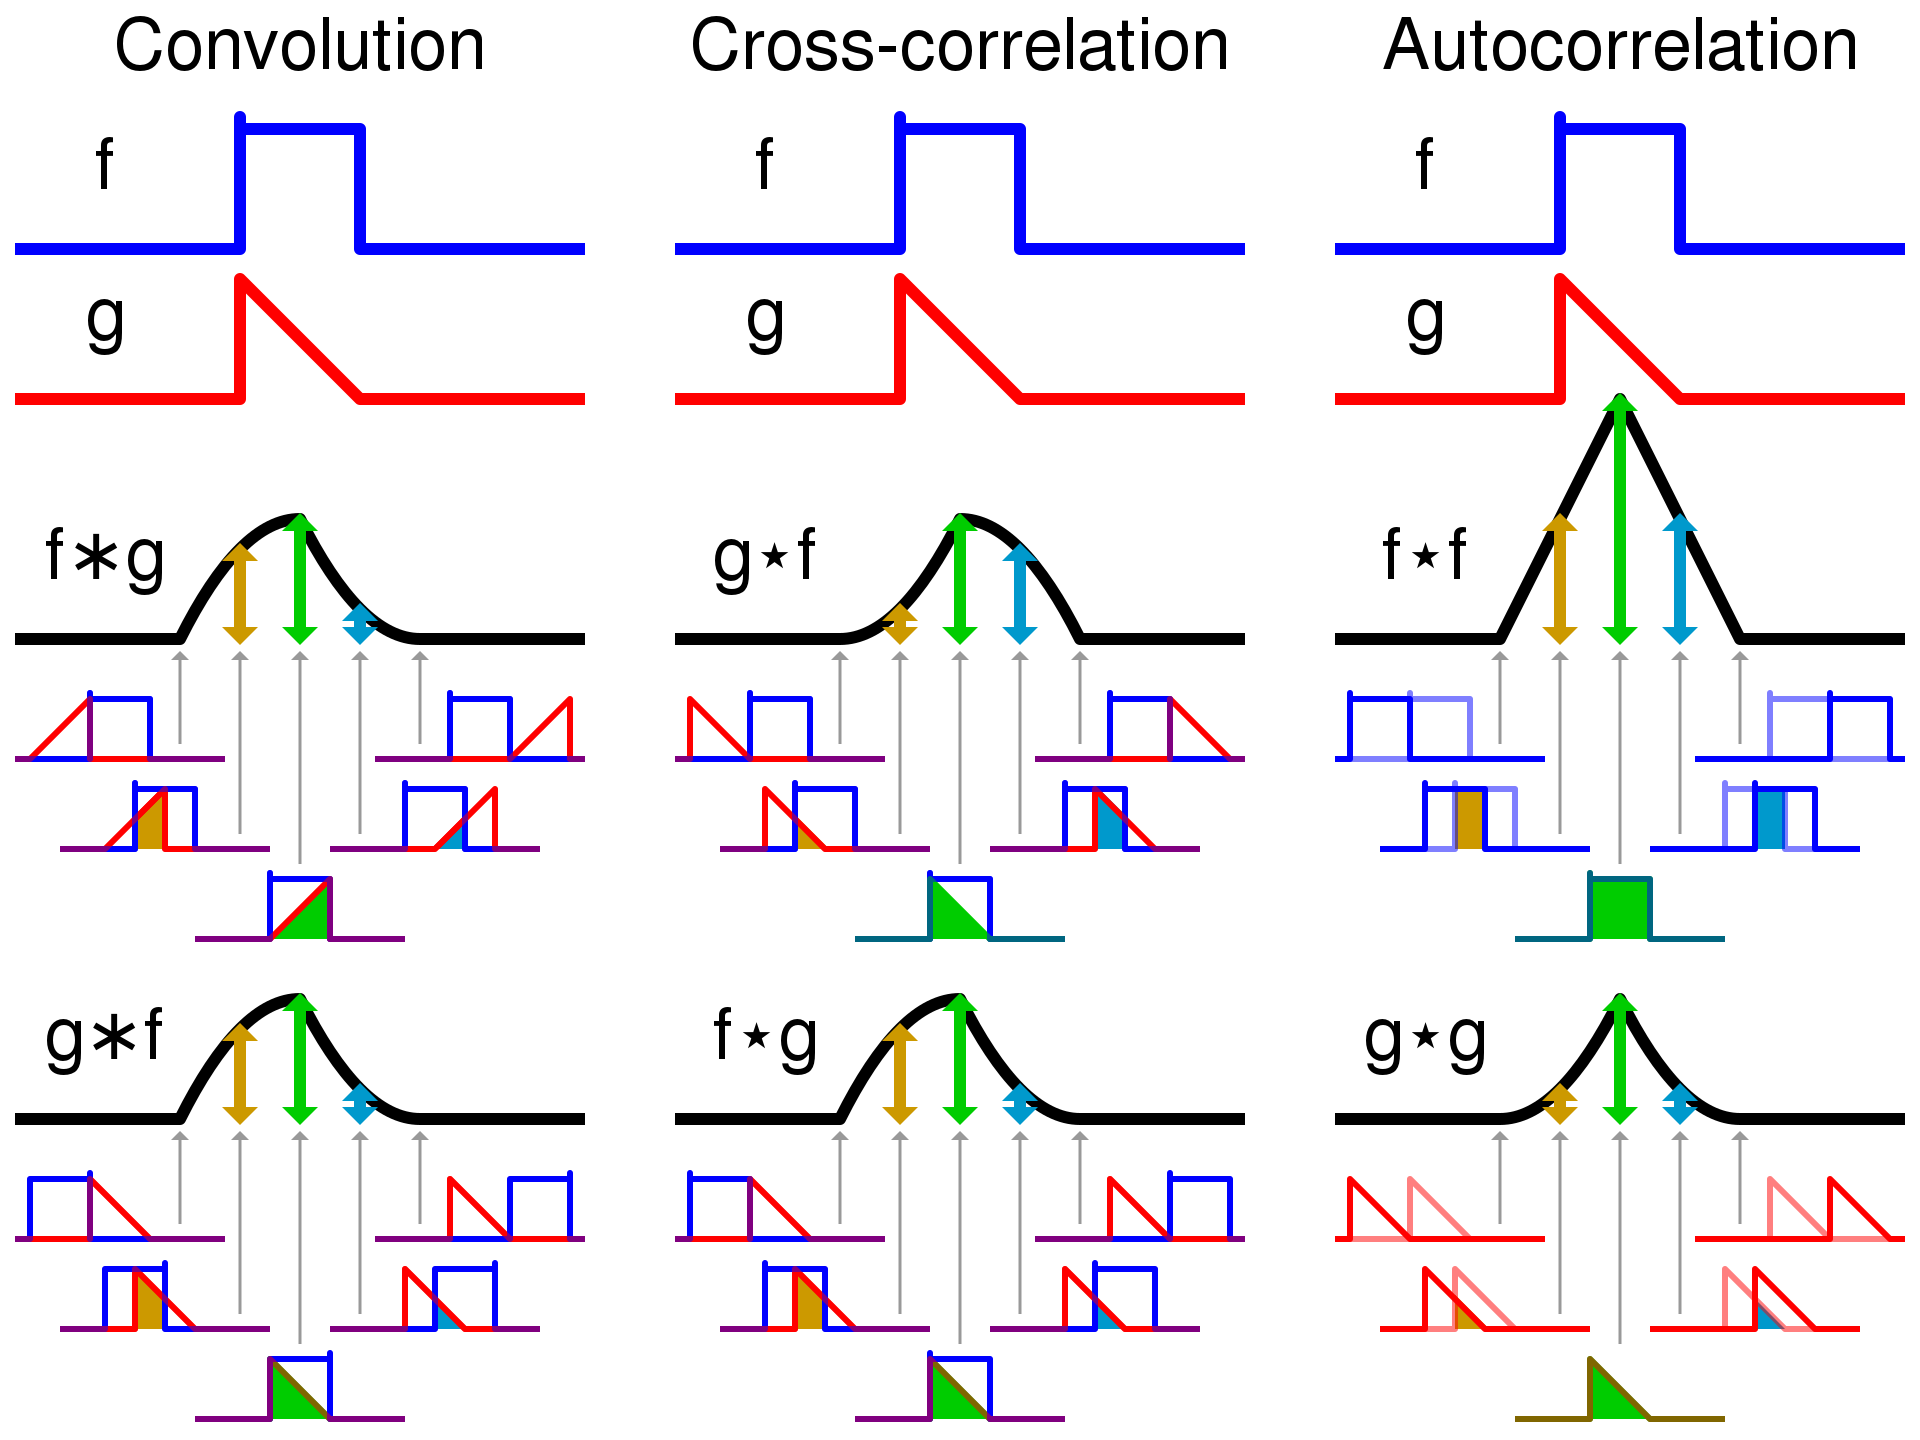
\includegraphics[width=.3\textwidth, trim={0 0 9in 0}, clip]{Comparison_convolution_correlation}
      \caption{Convolution versus cross-correlation. {\tiny Source: \url{https://en.wikipedia.org/wiki/Convolution}}}
    \end{figure}
    }
    \pause

    If the kernel is symmetric (which it is in practice), then cross-correlation and convolution are equivalent.
\end{frame}

\begin{frame}
  \frametitle{Convolution example}
  \pause
  Here, we compute $(K*I)(2,3)$ with $M = 3$ and $N = 3$ ($3\times 3$ kernel) \pause
  
    \visible<+->{
    \begin{figure}
      \centering
      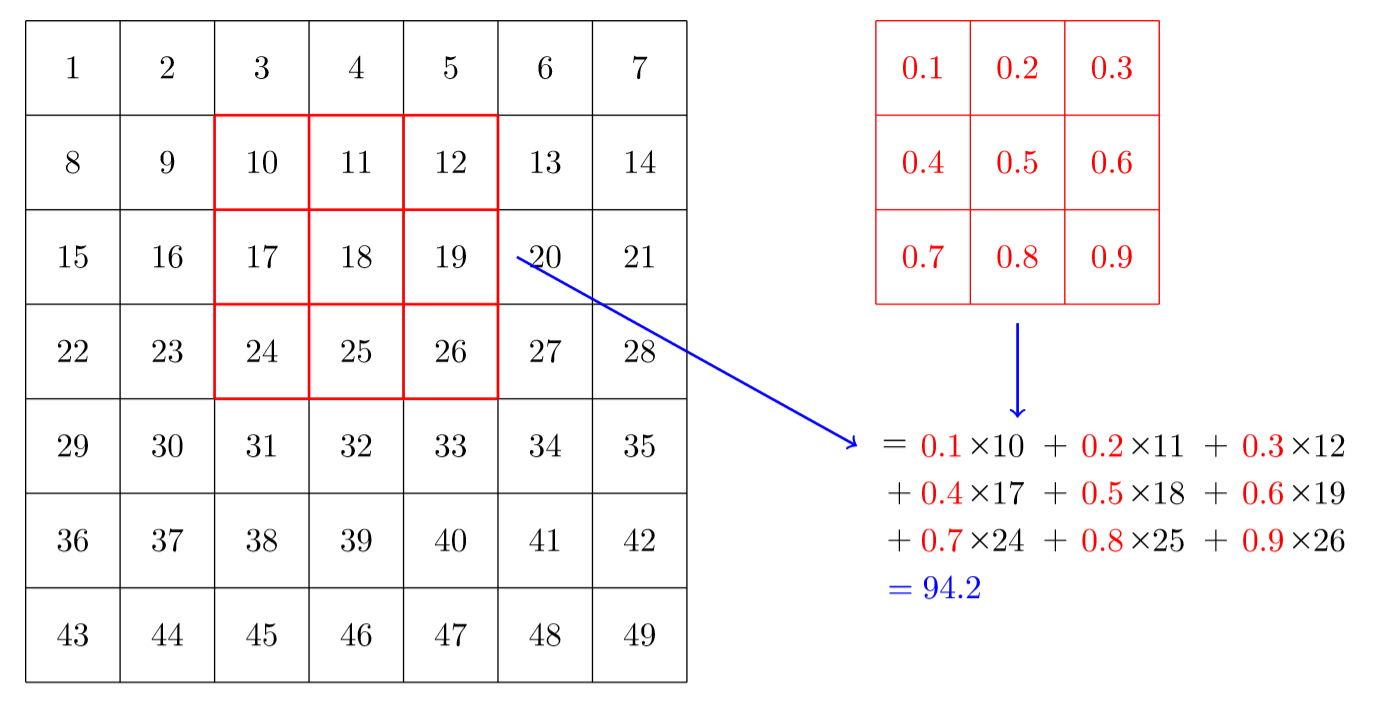
\includegraphics[width=.45\textwidth]{art4_one_conv}
      
      {\tiny Source: \url{https://sgugger.github.io/convolution-in-depth.html}}
      \end{figure}
    }
    \pause
    \begin{eqnarray*}\small
      (K*I)(2,3) &=& \pause \sum_{m=0}^{2}\sum_{n=0}^{2}I(2+m, 3+n)K(m,n) \\\pause
                 &=& \sum_{m=0}^{2}\Big[I(2+m, 3)K(m,0)\\
                 && \quad\quad + ~ I(2+m, 4)K(m,1) \\
                 && \quad\qquad + ~ I(2+m, 5)K(m,2)\Big]
    \end{eqnarray*}
\end{frame}

\begin{frame}
  \frametitle{Zero-padding}\pause
\begin{itemize}
  \item Convolving an $f_h \times f_w$ filter over an image of size $x_h \times x_w$ produces an output of size $(x_h -f_h + 1)\times (x_w - f_w +1)$ (\textbf{valid convolution})\pause
  \item But this reduces the spatial dimensions of the image at each layer\pause
  \item To preserve spatial dimensions, \textbf{zero-padding} is used: adding zeros around the border of the input image (\textbf{same convolution})\pause
  \item Thus, for an input of size $x_h \times x_w$, adding padding of size $p_h$ and $p_w$ results in an output of size $(x_h - f_h + 2p_h + 1)\times (x_w - f_w + 2p_w + 1)$\pause
\end{itemize}
  

\end{frame}



\begin{frame}
  \frametitle{Striding}\pause

  Striding refers to the step size $s$ with which the kernel moves across the input image. \pause
  \begin{itemize}[<+->]
    \item   Striding is used to reduce redundancy and thus speed up computation.
  \item A stride of 1 means the kernel is applied to every possible position.
  \item A stride of 2 means the kernel is applied every other position, effectively downsampling the feature map.
  \end{itemize}
  \pause
  Thus, given an input of size $x_h \times x_w$ and kernel size of $f_h \times f_w$, if we use a zero-padding of $p_h$ and $p_w$ and strides of $s_h$ and $s_w$, then the output has size:\pause

  \begin{equation}
    \lfloor \fr{x_h - f_h + 2p_h +s_h}{s_h}\rfloor \times \lfloor \fr{x_w - f_w + 2p_w +s_w}{s_w} \rfloor
  \end{equation}
\end{frame}


\section{CNN structure}
\begin{frame}
  \frametitle{Example structure of a CNN}\pause
  Convolutional layers enable the encoding of spatial relationships between neurons (pixels)\pause
  \begin{itemize}
  \item Weight sharing reduces number of parameters (i.e.\ same kernel/filter used for each feature map)\pause
  \item Complexity handled by increasing feature maps\pause
  \item Multiple convolutional layers can be stacked to add depth
  \end{itemize}
  \pause
  \visible<+->{
  \begin{center}
    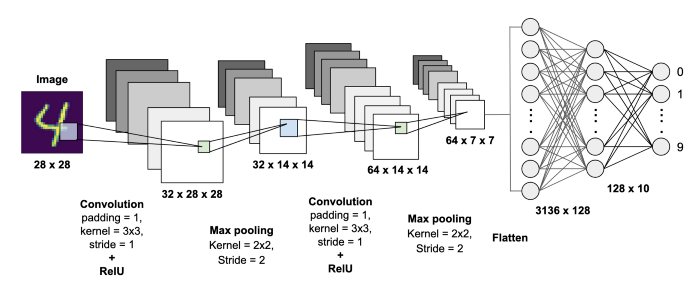
\includegraphics[width=.9\textwidth]{cnn-ex2}
  \end{center}
  {\tiny Source: \url{https://towardsdatascience.com/mnist-handwritten-digits-classification-using-a-convolutional-neural-network-cnn-af5fafbc35e9}}}
\end{frame}


\begin{frame}
  \frametitle{Convolutional layer}
  \pause
  The convolutional layer consists of several filters (kernels), each corresponding to a feature map. 

  \begin{itemize}
  \item Input: tensor of size $h_{1}\times w_{1} \times d_{1}$
    \begin{itemize}
    \item For the first convolutional layer: $d_{1} = 1$ (single-channel/grayscale image); $D_{1}=3$ (color/RGB image)
    \end{itemize}
    \pause
  \item Hyperparameters: \pause
    \begin{itemize}
    \item number of filters $F$
    \item kernel size (local receptive field) $f_h, f_w$
    \item stride length $s$
    \item amount of zero padding $p$ (typically same on both sides)
    \end{itemize}
    \pause
  \item Output: tensor of size $h_{2}\times w_{2}\times d_{2}$:\pause
    \begin{itemize}
    \item $h_{2} = (h_{1} - f_h + 2p + s)/s$
    \item $w_{2} = (w_{1} - f_w + 2p + s)/s$
    \item $d_{2} = F$
    \end{itemize}
  \end{itemize}
\end{frame}

\begin{frame}
  \frametitle{Example: Convolutional layer operation}
  \pause
  $d_{1} = 3$ (3-channel input) and $F = 2$ (2 filters). \pause

  \visible<+->{
    \centering
    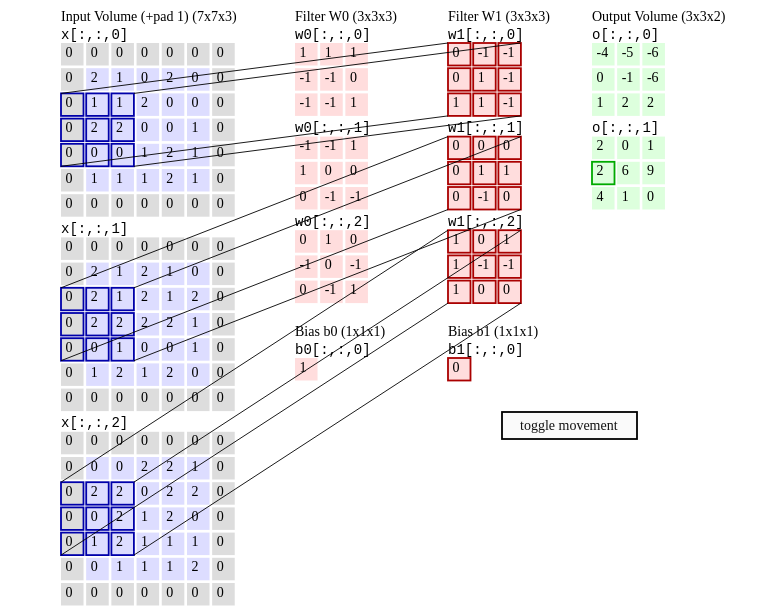
\includegraphics[width=.7\textwidth]{convolution}
    
    {\tiny Source: \url{https://cs231n.github.io/convolutional-networks/} (animated)}
  }
\end{frame}

\begin{frame}
  \frametitle{Pooling layer}
  \pause
  Pooling spatially downsamples the output of a convolutional layer via a summary statistic of nearby values at a given location
  \pause
  \begin{itemize}
  \item Introduced to ensure shift/translation invariance in a trained network\pause
  \item Leads to robust performance\pause
  \item Typically, \textbf{max} pooling or \textbf{average} pooling is used
  \end{itemize}
  \pause
  \visible<+->{
    \centering
    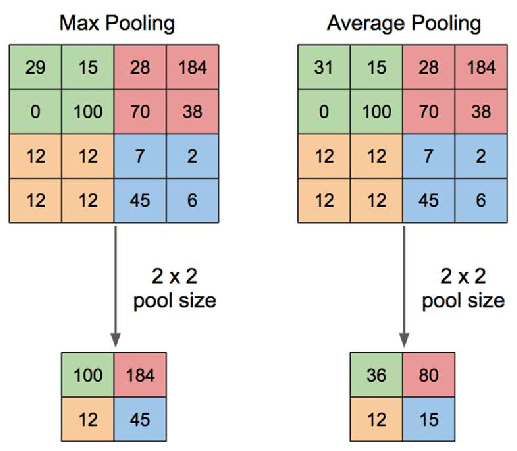
\includegraphics[width=.4\textwidth]{pooling}
  }
\end{frame}

\begin{frame}
  \frametitle{Training hyperparameters in a CNN}
  Several decisions must be made in selecting hyperparameters for training a CNN.

  \begin{itemize}[<+->]
  \item Number of convolutional layers and feature maps in each layer
  \item Convolutional kernel size
  \item Stride length (spacing of filters)
  \item Choice of pooling function (max, average, etc)
  \item Number of dense layers
  \item Activation function in each layer (ReLU, tanh, etc)
  \end{itemize}

 
\end{frame}

\begin{frame}
  \frametitle{Normalization layers}\pause
  Normalization layers are often used to improve training performance and stability. \pause
  \begin{itemize}
    \item Batch Normalization (BN): normalizes activations within a mini-batch
    \begin{eqnarray*}
      \tilde{\bm z}_n &=& \bm\gamma \odot \hat{\bm z}_n + \bm\beta, \quad \hat{\bm z}_n = \frac{\bm z_n - \bm\mu_{\text{batch}}}{\sqrt{\bm\sigma_{\text{batch}}^2 + \eps}}
    \end{eqnarray*}
    \item Layer Normalization (LN): normalizes across features for each training example
    \item Instance Normalization (IN): normalizes across spatial dimensions for each channel
  \end{itemize}

  

\end{frame}
\section{Architectures}
\begin{frame}
  \frametitle{CNN architectures for classification}
  \pause

   Various high-performing deep architectures have been developed in recent years that can be adapted for other problems: \pause
  
   \begin{itemize}[<+->]
   \item \href{http://vision.stanford.edu/cs598_spring07/papers/Lecun98.pdf}{LeNet}
  \item \href{https://papers.nips.cc/paper/2012/file/c399862d3b9d6b76c8436e924a68c45b-Paper.pdf}{AlexNet}
  \item \href{https://arxiv.org/abs/1409.1556}{VGGNet}
  \item \href{https://arxiv.org/abs/1512.03385}{ResNet}
  \item \href{https://static.googleusercontent.com/media/research.google.com/en//pubs/archive/43022.pdf}{Inception}
  \end{itemize}
  
\end{frame}

\begin{frame}
  \frametitle{LeNet-5}
  \pe
  \begin{itemize}[<+->]
  \item Created by Yann LeCun in 1998
  \item 5 convolutional layers
  \item Developed to classify handwritten digits (technology adopted by USPS and banks)
  \end{itemize}
  \pe
  \begin{center}
    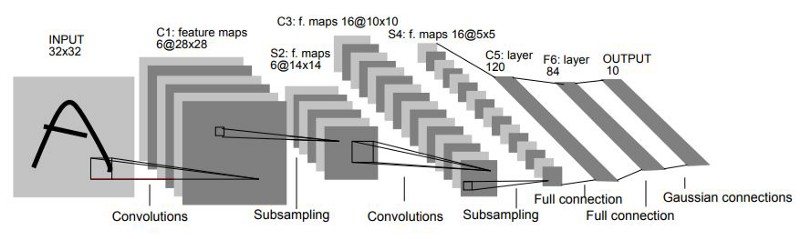
\includegraphics[width=.7\textwidth]{lenet-5}

    {\tiny Source: \url{https://www.datasciencecentral.com/lenet-5-a-classic-cnn-architecture/}}
  \end{center}
\end{frame}

\begin{frame}
  \frametitle{AlexNet}
  \pe
  \begin{itemize}[<+->]
  \item ReLU activations instead of tanh
  \item Dropout (instead of weight decay)
  \item Stacking of convolutional layers for larger receptive fields
  \end{itemize}
  \pe
  \begin{center}
    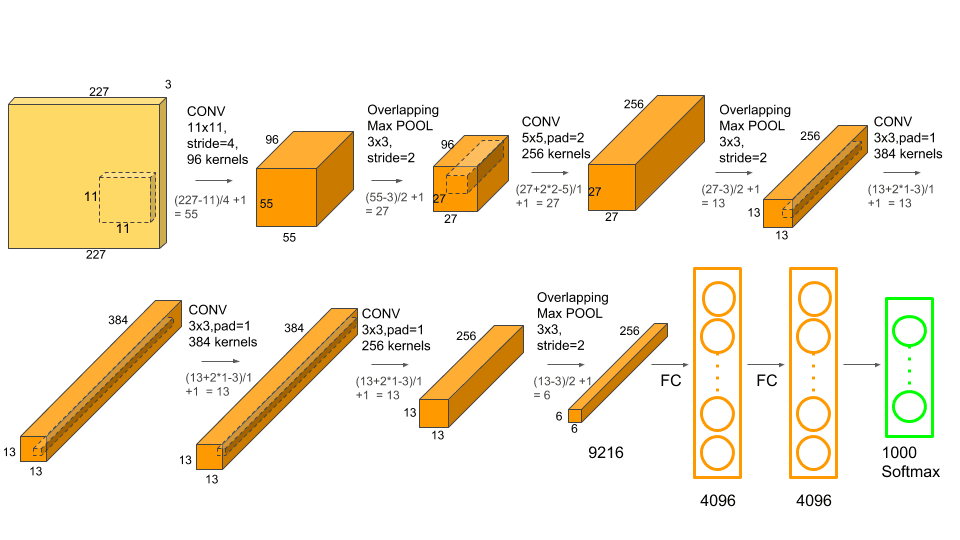
\includegraphics[width=.8\textwidth]{AlexNet-1}

    {\tiny Source: \url{https://neurohive.io/en/popular-networks/alexnet-imagenet-classification-with-deep-convolutional-neural-networks/}}
  \end{center}
\end{frame}

\begin{frame}
  \frametitle{VGGNet}
  \pe
  \begin{itemize}[<+->]
  \item Developed by Visual Geometry Group at Oxford
  \item Smaller receptive fields than AlexNet
  \item 16-19 layers deep
  \end{itemize}
  \pe
  \begin{center}
    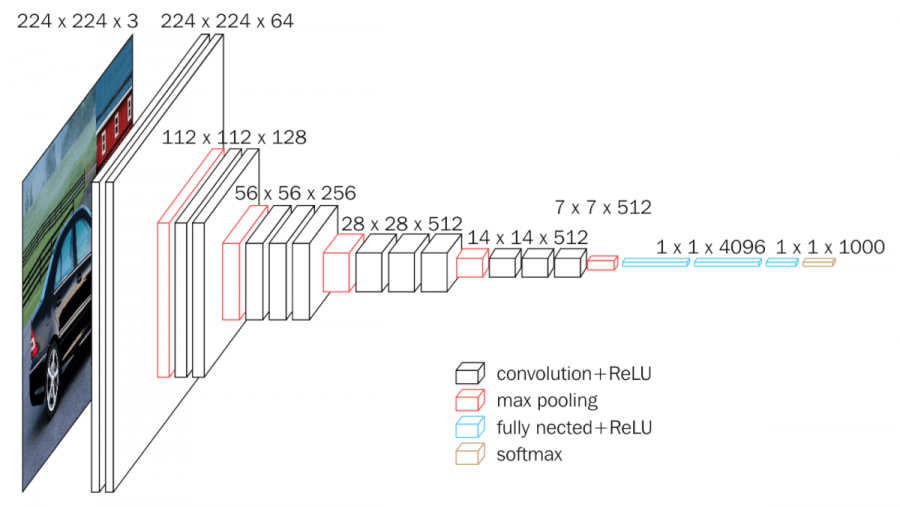
\includegraphics[width=.5\textwidth]{vgg}

    {\tiny Source: \url{https://www.kaggle.com/code/blurredmachine/vggnet-16-architecture-a-complete-guide}}
  \end{center}
\end{frame}

\begin{frame}
  \frametitle{ResNet}
  \pe
  \begin{itemize}
  \item Residual blocks: training nonlinear layer $\mc{F}$ to fit residual:\pe
    \begin{equation}
      \bm x_{\ell + 1} = \varphi(\bm x_{\ell} + \mc{F} (\bm x_{\ell}))
    \end{equation}\pe
    instead of total output:\pe
    \begin{equation}
      \bm x_{\ell + 1} = \mc{F} (\bm x_{\ell})
    \end{equation}
    \pe
  \item The introduction of skip connections allow for very deep networks (e.g.\ up to 1001 layers)
  \end{itemize}
  \pe
  \begin{center}
    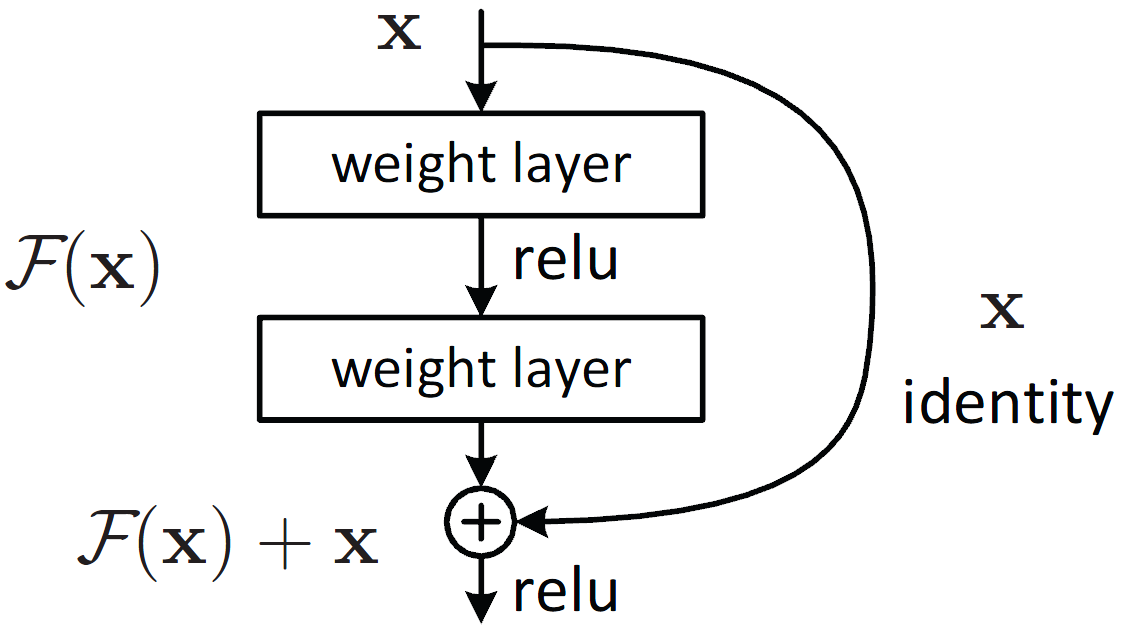
\includegraphics[width=.5\textwidth]{residual-block}

    {\tiny Source: \url{https://paperswithcode.com/method/residual-connection}}
  \end{center}
\end{frame}

\begin{frame}
  \frametitle{Inception (GoogLeNet)}
  \pe
  \begin{itemize}[<+->]
  \item First introduction of inception module (v1)
  \item Allows for multiple filter sizes at the same level
  \item $1\times 1$ convolutions reduce dimensionality (channels)
  \end{itemize}
  \pe
  \begin{center}
    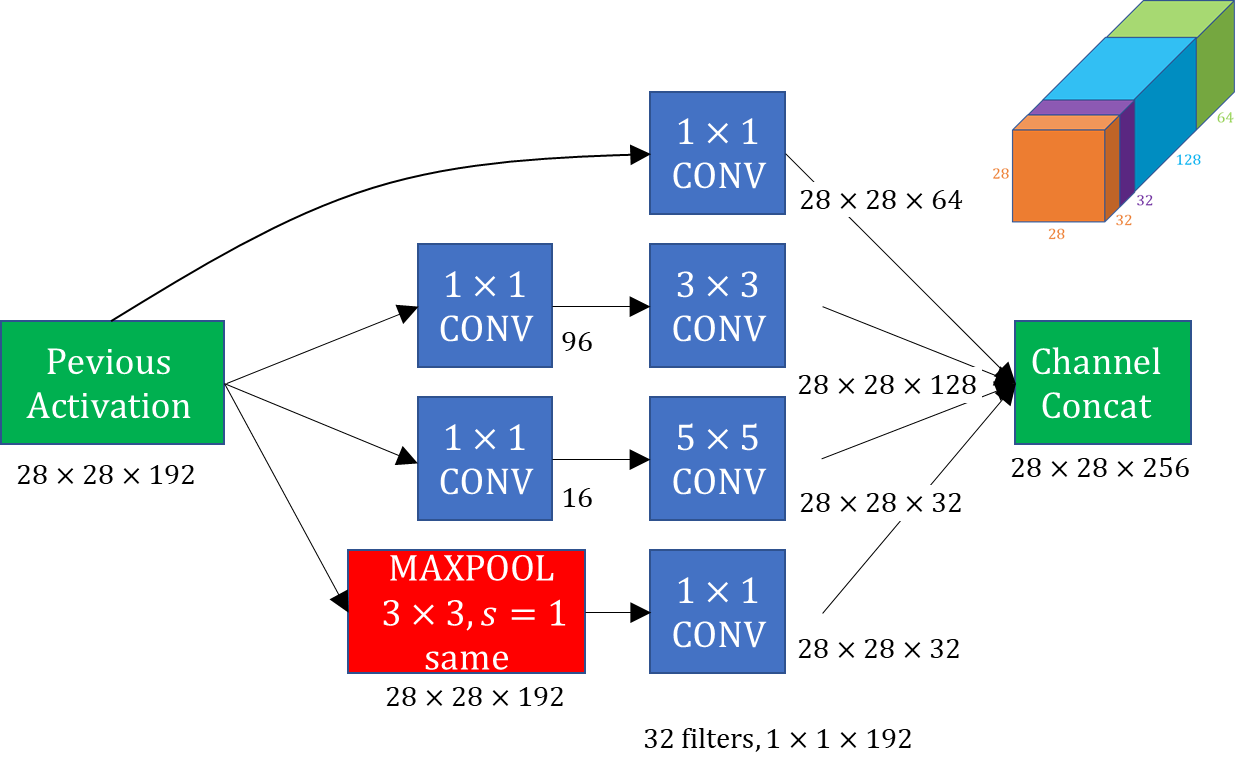
\includegraphics[width=.5\textwidth]{inception-module.png}

    {\tiny Source: \url{https://datahacker.rs/building-inception-network/}}
  \end{center}
\end{frame}

\section{Other  tasks}
\begin{frame}
  \frametitle{Image tagging}
  \pe
  \begin{itemize}[<+->]
  \item Assign multiple labels to single image (multi-label prediction; each tag predicted independently)\pe
  \item Output space: $\mc{Y} = \{0,1\}^C$, where $C$ is the number of tag types \pe
  \item Final layer of CNN has logistic sigmoid units (activations) instead of softmax
  \end{itemize}
  \pe

  \begin{center}
    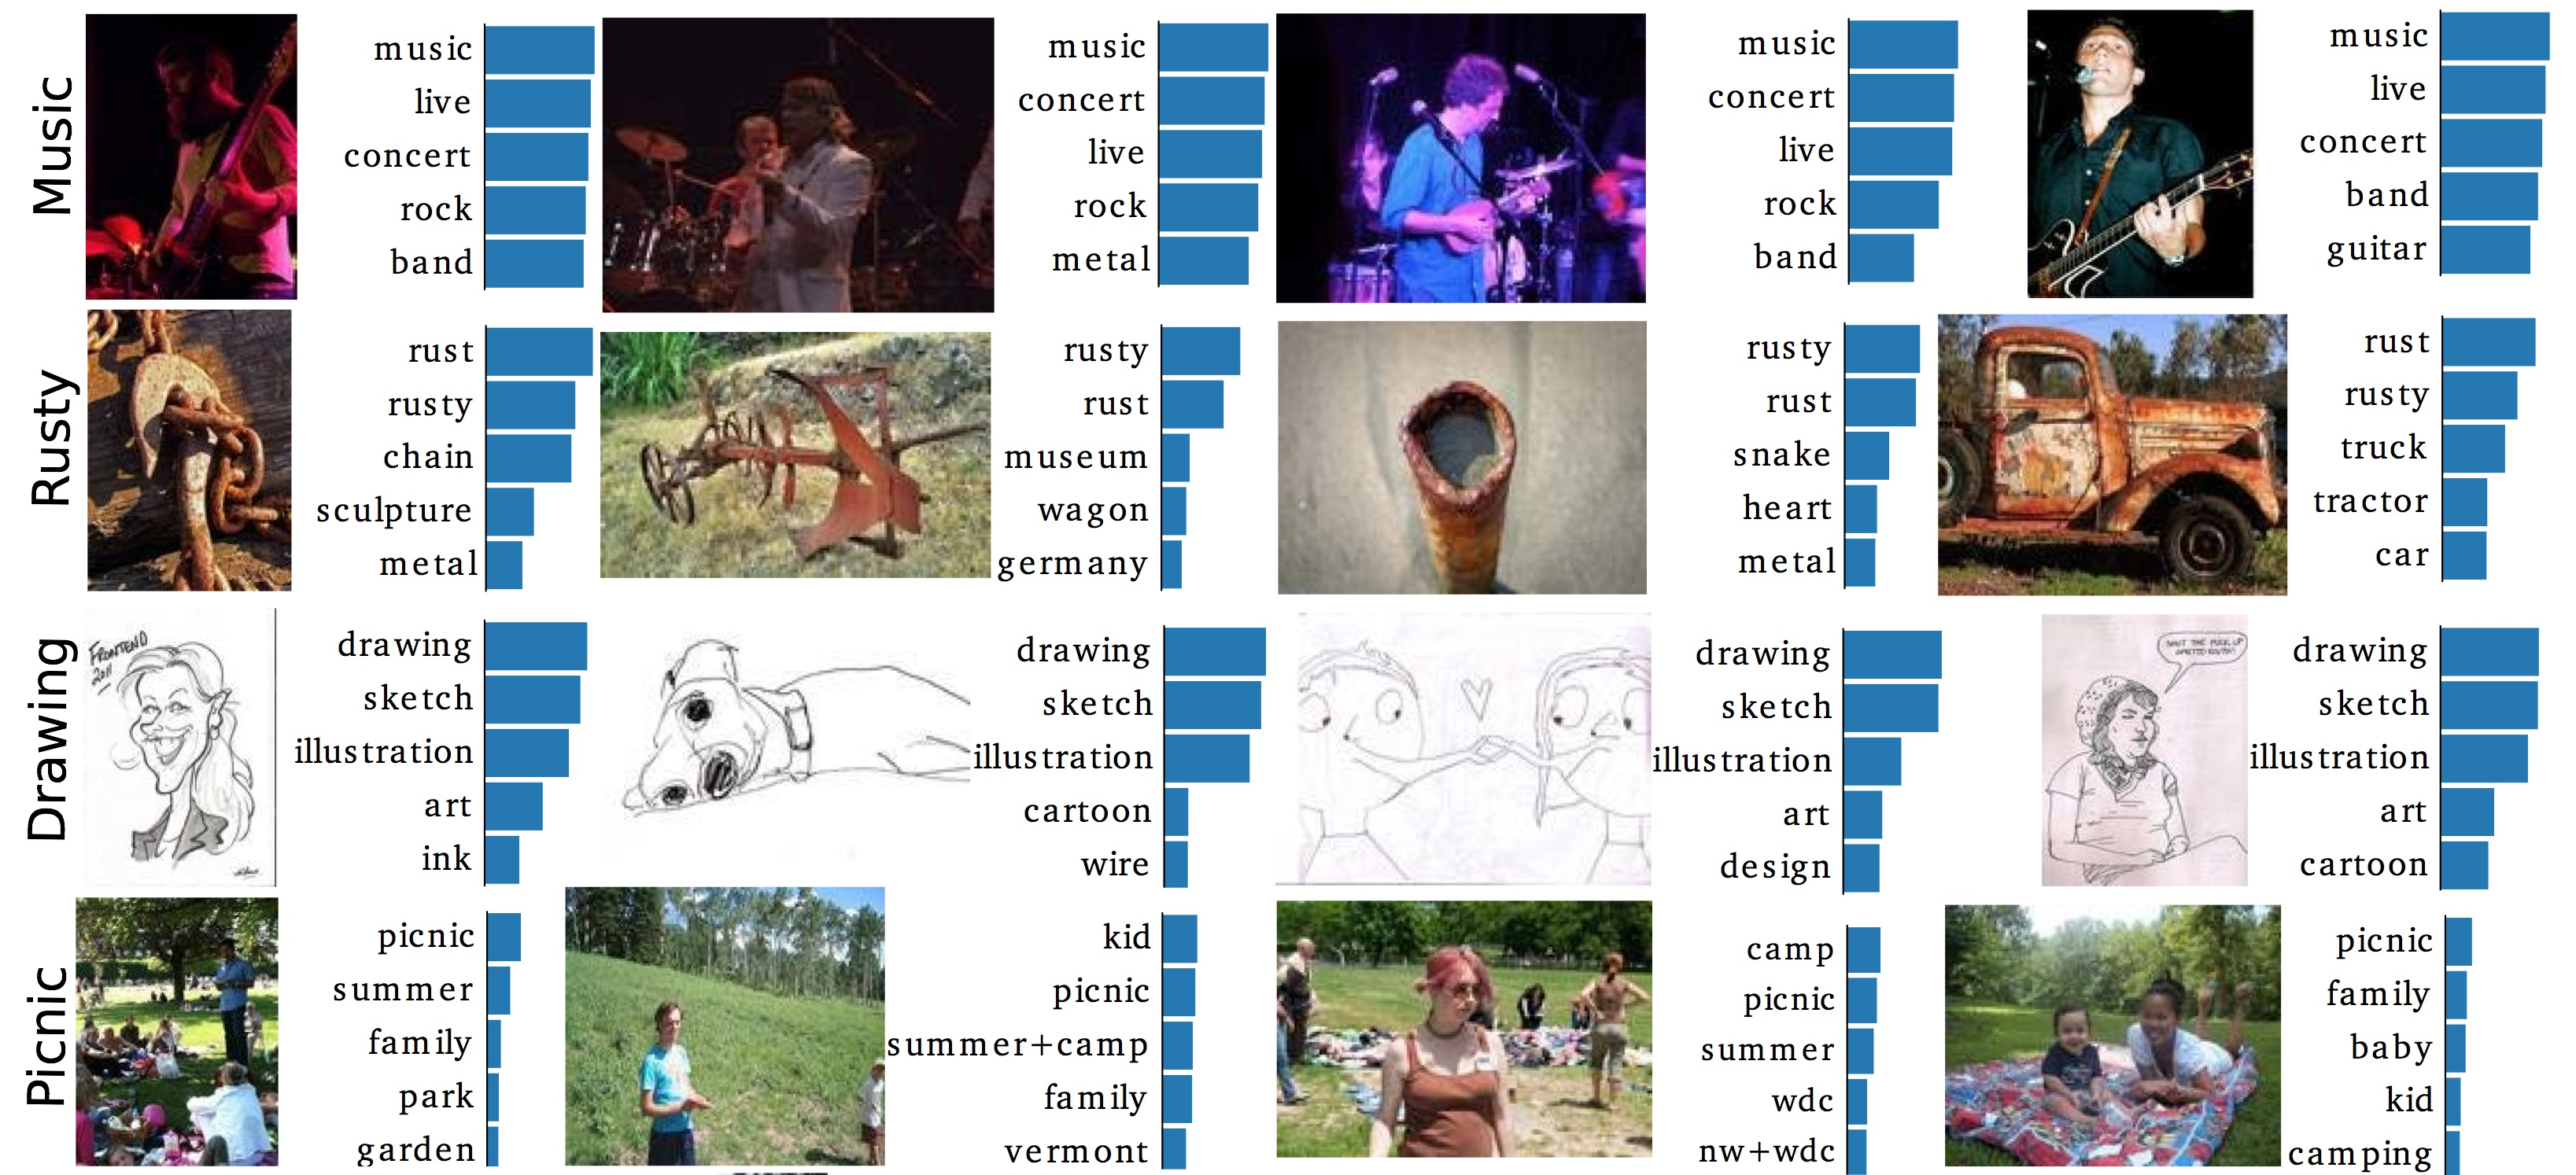
\includegraphics[width=.7\textwidth]{photoTagging1.jpg}

    {\tiny Source: \url{https://izadinia.github.io/files/DeepTagging-mmcommons.pdf}}
  \end{center}
  
\end{frame}


\begin{frame}
  \frametitle{Object detection}
  \pe
  \begin{itemize}
  \item Variable number of objects of interest in a given image (open world problem) \pe
  \item Returns set of labeled bounding boxes around objects of interest \pe
  \item Popular models for object detection: \pe
    \begin{itemize}
    \item \href{https://arxiv.org/pdf/1506.02640.pdf}{YOLO} (You Only Look Once)\pe
    \item \href{https://arxiv.org/pdf/1512.02325.pdf}{SSD} (Single shot detector)\pe
    \end{itemize}
  \end{itemize}

  
  \begin{center}
    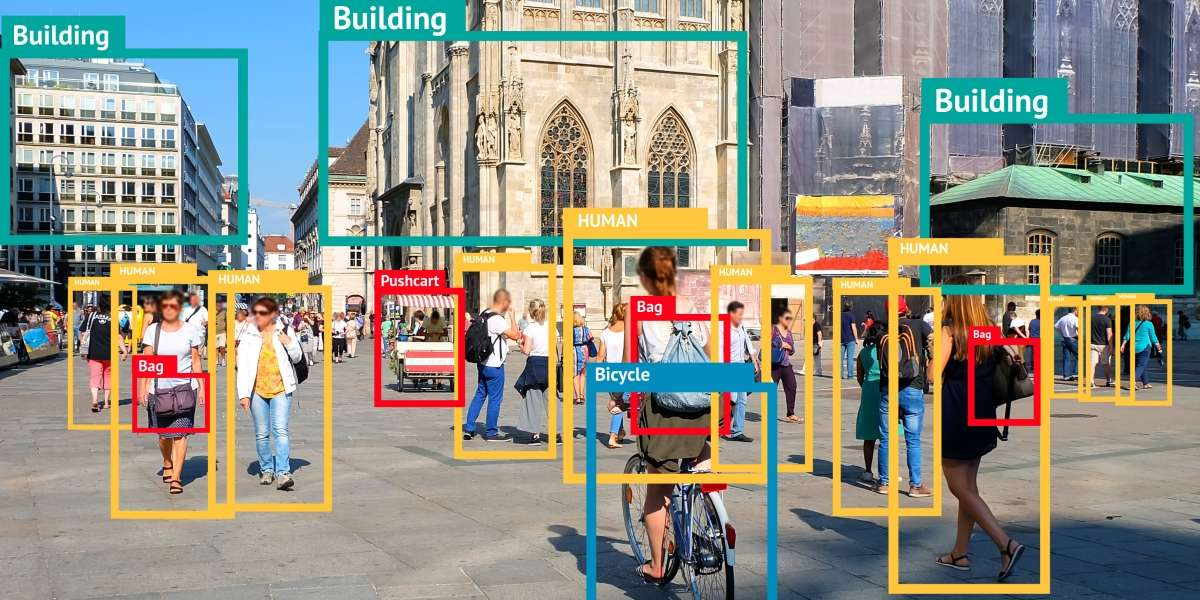
\includegraphics[width=.7\textwidth]{YOLO.jpg}

    {\tiny Source: \url{https://aigeekprogrammer.com/yolo-fast-object-detection-and-classification/}}
  \end{center}
  
\end{frame}


\begin{frame}
  \frametitle{Semantic segmentation}
  \pe
  \begin{itemize}
  \item Predicts a class label for each pixel rather than an image, e.g. $y_i \in \{1,\ldots,c\}$ where 1$\equiv$sky, 2$\equiv$sheep, 3$\equiv$grass, etc \pe
  \item Achieved via encoder-decoder network (captures high-level features in 2D bottleneck)\pe
  \item Popular model: \href{https://link.springer.com/chapter/10.1007/978-3-319-24574-4_28}{U-Net}\pe
  \end{itemize}

      
    \begin{minipage}[h]{.6\linewidth}
    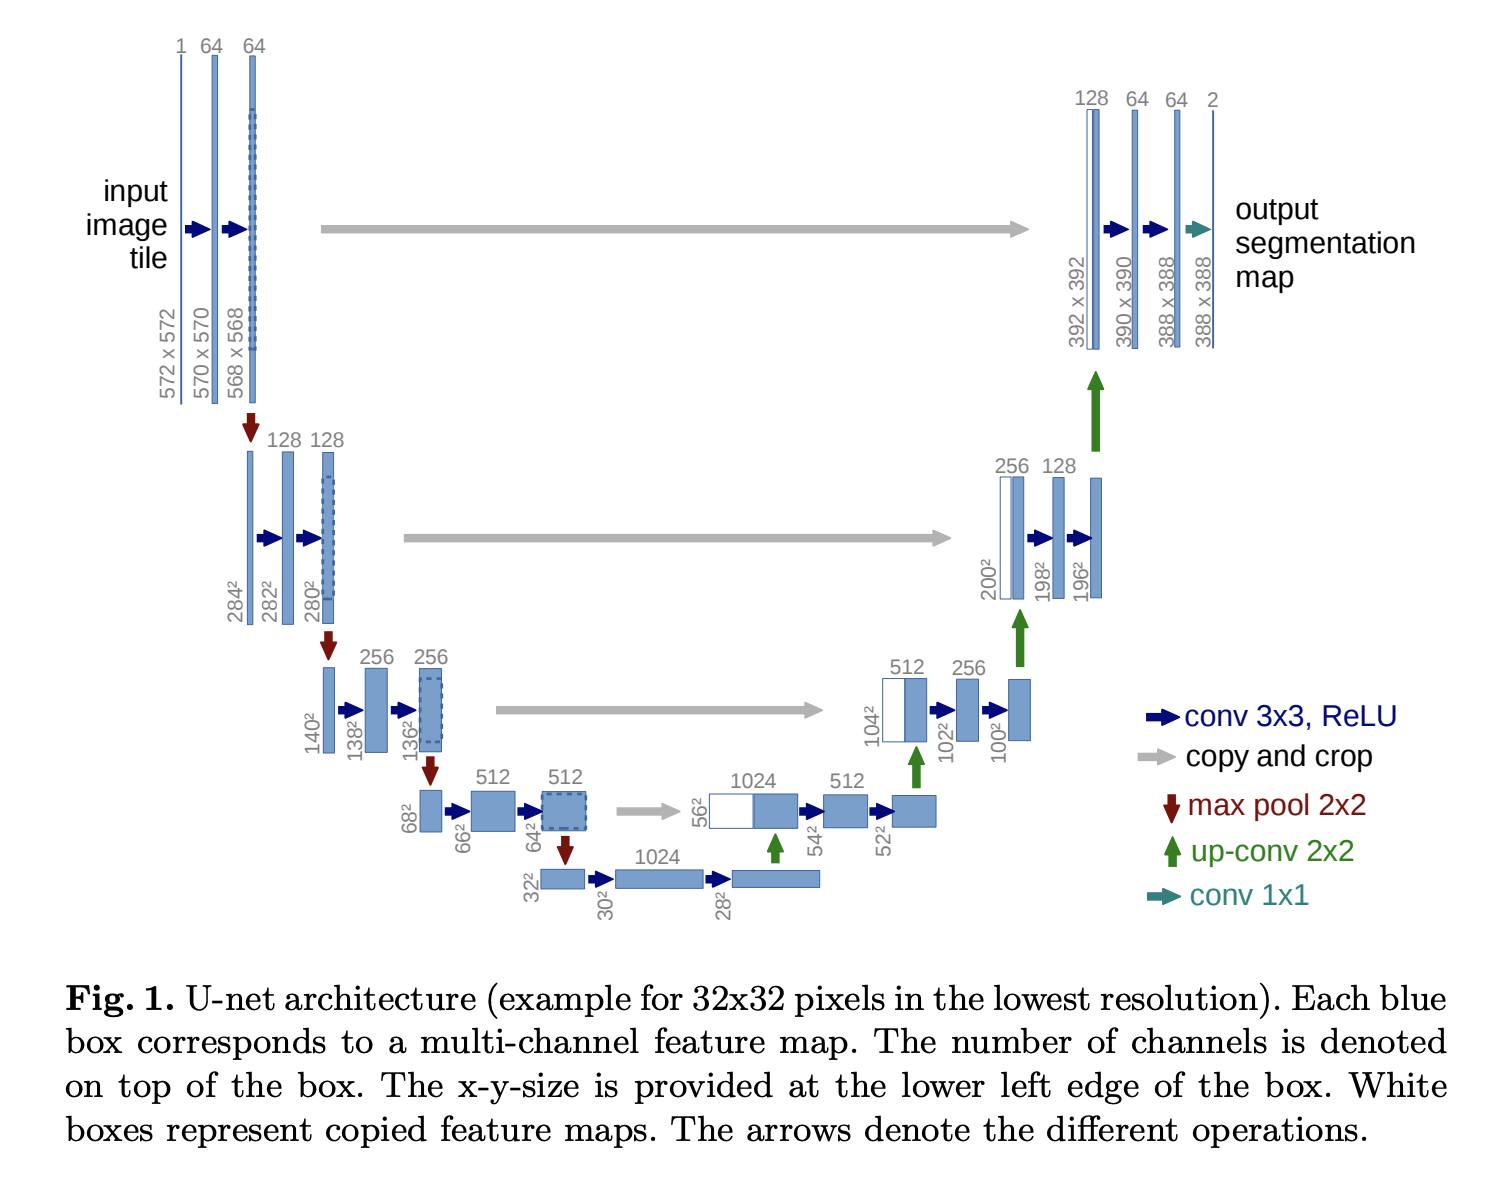
\includegraphics[width=\textwidth]{unet-architecture-paper}

    {\tiny Source: \url{https://paperswithcode.com/method/u-net}}      
    \end{minipage}
    \begin{minipage}[h]{.36\linewidth}
      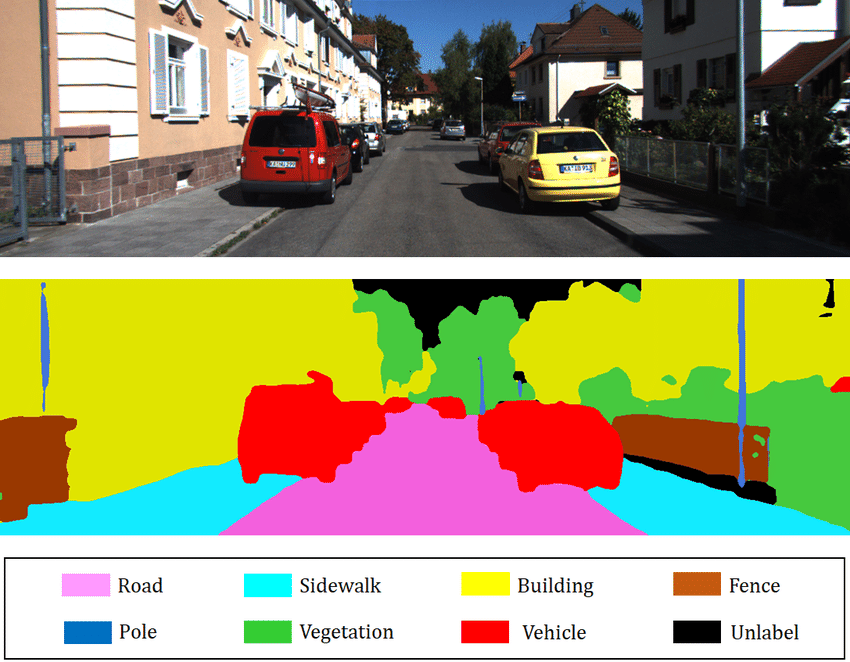
\includegraphics[width=\textwidth]{segmented-image}
      \raggedright
    {\tiny Source: \url{https://towardsai.net/p/l/machine-learning-7}}
    \end{minipage}
 

  
\end{frame}


\begin{frame}
  \frametitle{Instance segmentation}
  \pe

  \begin{itemize}
  \item Combines object detection and semantic segmentation\pe
    \item For object instance, a \textit{2d shape mask} is predicted instead of the bounding box\pe
  \item Achieved by applying \textbf{semantic segmentation} to each detected box in order to label each pixel
    as foreground or background\pe
  \item Popular models: \pe
    \begin{itemize}
    \item \href{https://arxiv.org/pdf/1703.06870.pdf}{Mask R-CNN}\pe
    \item \href{https://arxiv.org/pdf/1506.01497.pdf}{Faster R-CNN}
    \end{itemize}
  \end{itemize}
  \pe

    
  \begin{center}
    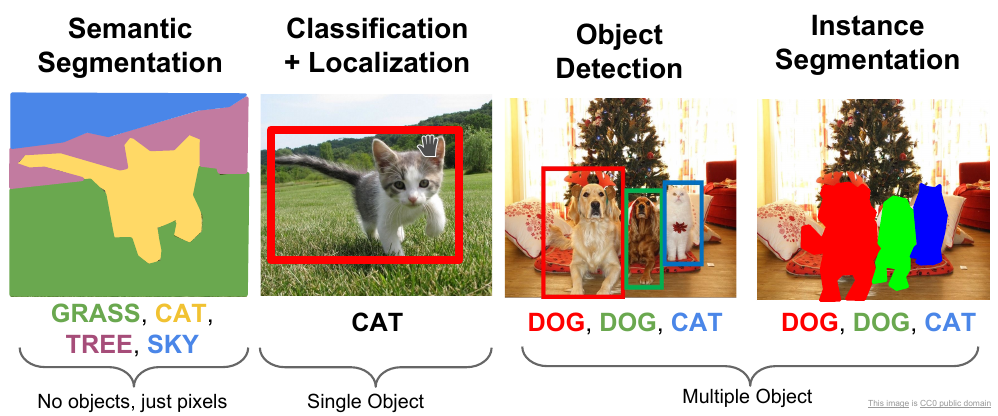
\includegraphics[width=.7\textwidth]{segmentation}

    {\tiny Source: \url{https://kharshit.github.io/blog/2019/08/23/quick-intro-to-instance-segmentation}}
  \end{center}

\end{frame}

\begin{frame}
  \frametitle{Human pose estimation}
  \pe
  \begin{itemize}
  \item Predicts location of fixed set of skeletal keypoints (in 2D or 3D)\pe
  \item Popular models: \pe
    \begin{itemize}
    \item \href{https://link.springer.com/chapter/10.1007/978-3-030-01264-9_17}{PersonLab}\pe
    \item \href{https://arxiv.org/pdf/1812.08008.pdf}{OpenPose}
    \end{itemize}
  \end{itemize}

  \pe

    \begin{center}
    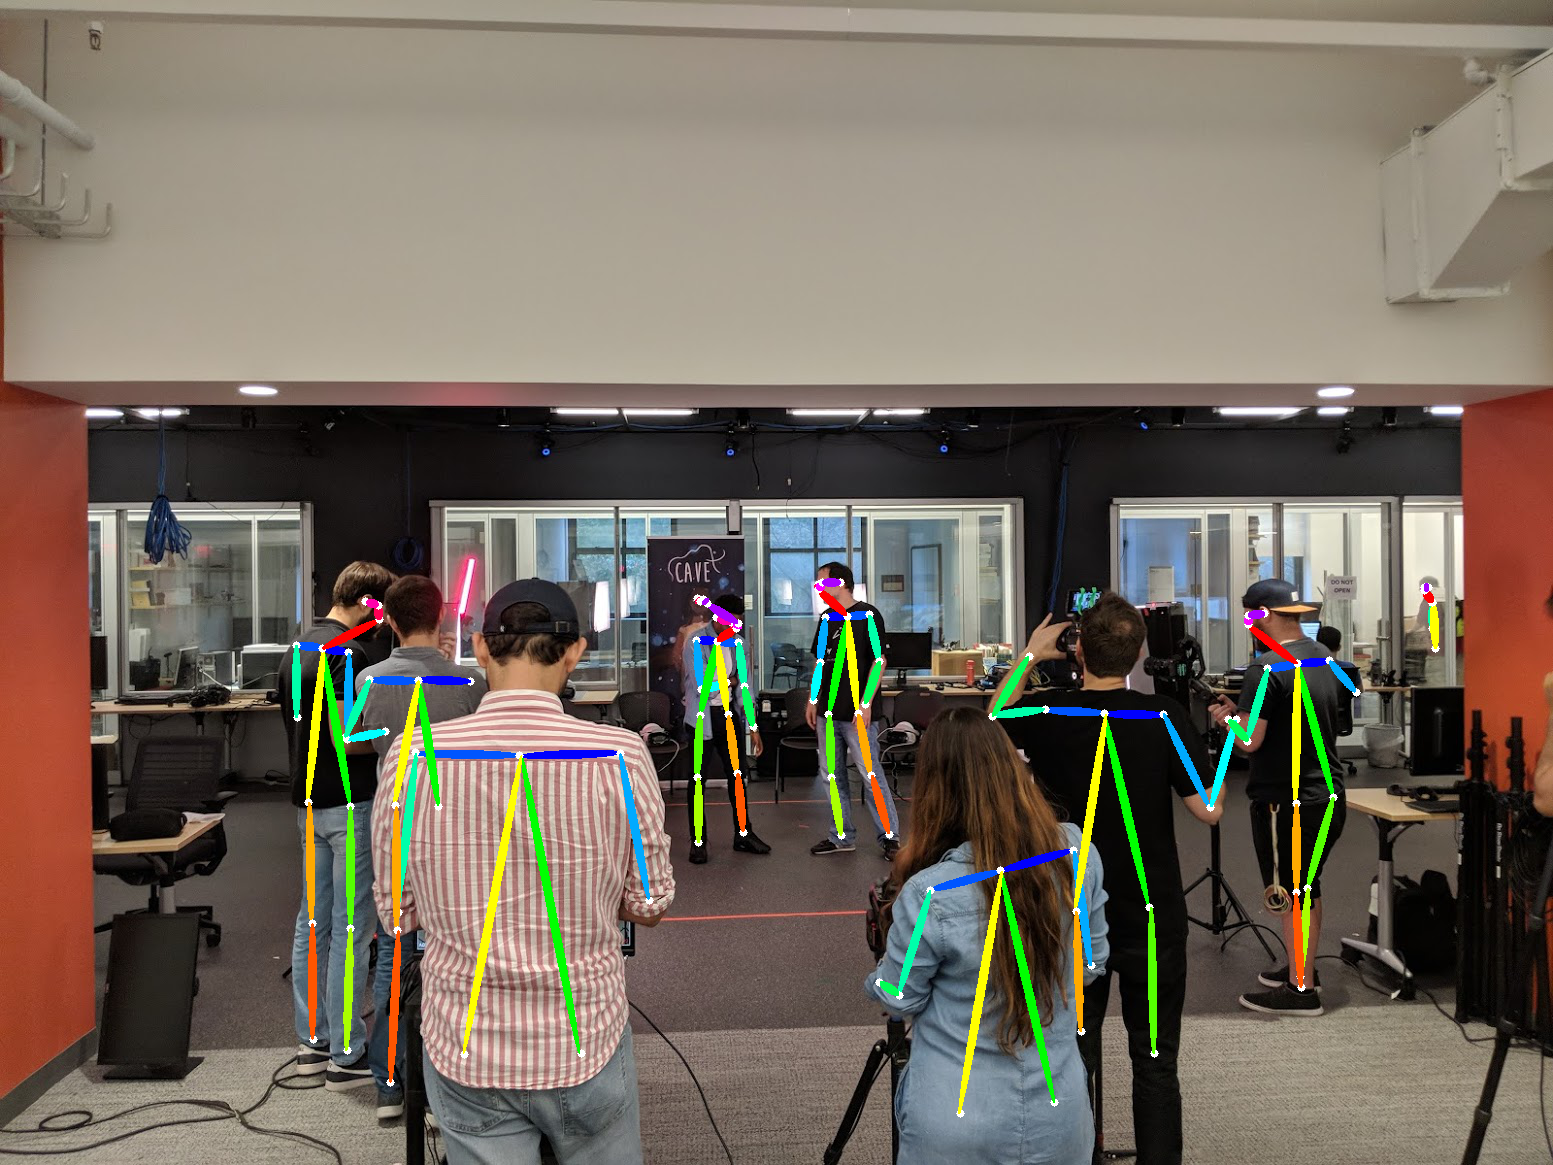
\includegraphics[width=.5\textwidth]{shoot1-pose}

    {\tiny Source: \url{https://frl.nyu.edu/tricking-openpose/}}
  \end{center}
  
\end{frame}

\section{Outlook}
\begin{frame}
  \frametitle{Summary}
  \begin{itemize}
  \item Basic convolutional neural networks for image classification consist of:
    \begin{itemize}
    \item input layer
    \item convolutional layers (multiple filters=feature maps)
    \item pooling layers
    \item dense/fully-connected layers
    \item output layer
    \end{itemize}
  \item Visualize and experiment with a CNN for handwritten digit recognition: \url{https://www.cs.ryerson.ca/~aharley/vis/conv/}
    \item Reading: \textbf{PMLI} 14; \textbf{DL} 9
  \end{itemize}
\end{frame}
 
\appendix

 
\end{document}

%%% Local Variables:
%%% mode: latex
%%% TeX-master: t
%%% End:
